\documentclass{article}

\usepackage[utf8]{inputenc}
\usepackage[T1]{fontenc}
\usepackage{hyperref}
\usepackage{url}
\usepackage{booktabs}
\usepackage{amsfonts}
\usepackage{nicefrac}
\usepackage{microtype}
\usepackage{amsmath}
\usepackage{amssymb}
\usepackage{graphicx}
\usepackage{algorithm}
\usepackage{algpseudocode}
\usepackage{tikz}
\usetikzlibrary{shapes,arrows,positioning}

\usepackage[margin=1in]{geometry}

\title{\textbf{Sentient Topology: Plasticity-Aware Affective Representation
in a Humanities-Grounded Sensory Associative Network}}

\author{
  \textbf{Hochanho} \\
  Independent Researcher \\
  Seoul, Republic of Korea \\
  ORCID: \href{https://orcid.org/0009-0002-3258-2466}{0009-0002-3258-2466} \\
  Code: \href{https://github.com/HocH88/sentient-topology}{github.com/HocH88/sentient-topology} \\
  \texttt{hochanho@example.com}
}

\date{}

\begin{document}

\maketitle

\begin{abstract}
Affective computing represents emotion using discrete labels or low-dimensional
coordinates (Valence--Arousal--Dominance). Human affect, in contrast, is
contextual, non-reductive, and topologically complex: what one feels is not a
singular label but a multi-faceted shape of associative network activation.
We present \textbf{Sentient Topology}, a framework that formalizes artificial
emotion as the topological shape of activation in a Humanities-Grounded
Sensory Associative Network (SAN), and extends it with a synaptic-plasticity
engine so that the shape evolves under repeated experience. The framework
contributes: (1) a SAN with an auditable composition of corpus PPMI edges,
rule-based active inhibition, and rule-based context-to-affect seed channels;
(2) a context-conditional, type-biased, degree-normalized spreading
activation; (3) a five-dimensional topological signature
$(D, S, C, H, B)$ whose Symmetry is the normalized algebraic connectivity of
the active subgraph and whose Boundary is computed by a self-contained
pure-Python $\mathbb{Z}_2$ persistent-homology solver; (4) a six-mechanism
plasticity engine (Hebbian, Habituation, Sensitization, Homeostatic Scaling,
Fading Affect Bias, Consolidation), each grounded in a specific
neuroscientific or affective-psychology literature; (5) a four-dimensional
\emph{motivation} vector (curiosity, resolve, express, deepen) derived from
the topological asymmetry, grounded in dopamine reward-prediction-error,
incentive-salience, effort-based decision-making, and curiosity-VTA-hippocampus
literature, providing a measurable Level-2 (intrinsic motivation) layer on
top of the Level-1 topological signature; (6) an instance isolation
principle ensuring that multiple SAN entities share code but never share
weights or feedback. Empirically, on an 8{,}000-node lemmatized SAN derived
from a balanced 200-work Project Gutenberg corpus ($\sim$22.3M tokens; six
categories: English classics 30\%, modernism 20\%, philosophy 20\%, eastern
classics 15\%, American literature 10\%, poetry 5\%), the same seed concept
produces topologically distinct shapes under contrasting contexts; an
ablation across three seeds shows that Depth and Boundary together carry
$\sim$88\% of context discrimination. We further introduce an
\emph{intra-corpus affect-trajectory differentiation} protocol: holding the
corpus fixed and parameterizing SAN propagation with Panksepp's seven
primary affect circuits (LUST excluded; six affects plus a uniform
baseline), we run $7 \times 6 = 42$ deterministic propagations across six
stimuli. Boundary emerges as the \emph{primary observable}, producing
systematically consistent directional differences for $13$ of $21$
affect pairs across at least four of six stimuli (no other dimension exceeds
six). A continuum from constriction (RAGE / FEAR / PANIC) through baseline
to expansion (PLAY / SEEKING / CARE) emerges on mean Boundary, matching
Panksepp's approach/avoidance classification as a suggestive analog. A
sensitivity analysis ($\pm 50\%$ on each affect parameter) identifies
exactly two \emph{brittle} channels (SEEKING.concept-bias and
CARE.proximity-weight) as the dominant effect channels of their affects;
thirteen other channels are robust and five are stimulus-conditional. We
further release a multi-phase scale-up roadmap from 200 to 5{,}000+ works
($\sim$500M tokens, NLP foundation-model scale). The plasticity engine
reproduces the Thompson--Spencer habituation curve, the Walker--Skowronski
Fading Affect Bias, and surprise-driven sensitization on the same SAN, with
effect sizes and signs consistent with the source literature. The framework
makes no claim of conscious felt experience and no claim to validate
Panksepp's affective neuroscience framework; what we report is the
topological signature that a committed affect $\to$ SAN parameter mapping
produces. We close with a honest
limitation: the rule-augmented inhibition and seed channels are reported as
augmentations rather than hidden under ``learned,'' and human-subject
validation of the topological signatures remains future work.
\end{abstract}

\section{Introduction}
The dominant paradigm of emotion modeling in artificial intelligence either
classifies affect into discrete labels or projects it onto low-dimensional
continuous spaces \cite{cowen2021semantic, fontaine2016modeling}. While
statistically useful, these representations exhibit a sharp gap with respect
to human affect, which is constructed dynamically in context and resists
singular categorization \cite{barrett2017theory}. Reading an old letter by a
rainy window does not evoke a single label of ``sadness''; it activates an
intricate mixture of longing, regret, warmth, resignation, and gratitude, and
the felt sense is not the sum of these parts but the holistic shape formed by
their co-activation. Drawing inspiration from Tononi's Integrated Information
Theory \cite{tononi2008qualia}, where qualia are formalized as a geometric
shape in a high-dimensional space, we propose that artificial emotion can be
modeled as the topological shape of an activated network.

Beyond a static formalism, a serious model of affect must address how a
network's response to a stimulus changes when the stimulus is encountered
repeatedly. Neuroscience has documented at least six relevant phenomena --
Hebbian co-activation \cite{hebb1949organization}, habituation
\cite{thompson1966habituation, rankin2009habituation}, sensitization
\cite{groves1970habituation}, homeostatic synaptic scaling
\cite{turrigiano2008homeostatic}, the asymmetric Fading Affect Bias
\cite{walker2009fab}, and sleep-driven consolidation
\cite{diekelmann2010memory} -- each of which is missing from current
emotion-representation pipelines. We integrate all six into a single
plasticity engine that operates on the same SAN as our static topology, so
the affective shape evolves under experience.

Our contributions are six-fold:
\begin{enumerate}
    \item A formal SAN with an explicit, auditable composition of
      (i)~corpus-derived PPMI edges over a category-balanced 200-work
      Project Gutenberg corpus ($\sim$22.3M tokens) spanning six categories
      (English classics 30\%, modernism 20\%, philosophy 20\%, eastern classics
      15\%, American literature 10\%, poetry 5\%),
      (ii)~a rule-based active-inhibition table between opposing sensations,
      and (iii)~a rule-based context-to-affect seed map. We do \emph{not}
      claim that (ii) and (iii) are learned; their finite tables are released
      with the artifact (\S 3.1).
    \item A five-dimensional topological signature
      $T = (D, S, C, H, B)$ whose Symmetry is the normalized algebraic
      connectivity ($\lambda_2$ of the normalized Laplacian) of the active
      subgraph and whose Boundary is the sum of $H_1$ persistence lifetimes,
      computed by a pure-Python $\mathbb{Z}_2$ solver with no external TDA
      dependency (\S 3.3, \S 4).
    \item A six-mechanism synaptic plasticity engine grounded in
      neuroscience and affective psychology, with hooks for additional
      invariant-preserving mechanisms described elsewhere and not claimed
      here (\S 3.4).
    \item Empirical validation on a 5{,}000-node lemmatized SAN
      ($\sim$4.35M tokens, forty-one literary works): a static case study
      with baselines and dimension-drop ablation, and three plasticity
      experiments reproducing habituation, Fading Affect Bias, and
      surprise-driven sensitization with effect signs and magnitudes
      consistent with the source literature (\S 5).
    \item An \textbf{instance isolation principle}: code is shared across
      SAN instances, but per-instance state (weights, activation logs,
      auxiliary configurations) is strictly isolated and feedback never
      crosses between instances (\S 6).
\end{enumerate}

We also report an \textbf{honest negative finding}: among the five topology
dimensions, Depth and Boundary jointly carry $\sim$88\% of the discriminative
signal across three seed concepts; Density, Symmetry, and Centrality together
contribute $\sim$12\%. We keep the five-dimensional formalism for theoretical
completeness, but the discriminative work is concentrated in the geodesic
and persistence-based invariants.

\section{Related Work}
\textbf{Topological Data Analysis in deep learning.} Persistent homology and
related TDA techniques have been used both as input features and as
regularizers for neural networks
\cite{bubenik2015statistical, zeng2024neural, hofer2017deep}. We borrow the
machinery but shift the target of analysis from the network's parameters or
embeddings to the topology of its \emph{induced active subgraph} under a
specific stimulus.

\textbf{Geometric and semantic models of emotion.} Classical valence-arousal
models, the 27-category space of \cite{cowen2017self}, and the 4D hypercube
of \cite{fontaine2016modeling} formalize the global landscape of affect.
Constructionist theory \cite{barrett2017theory, barrett2025more} emphasizes
that each affective instance is itself a constructed pattern. We treat each
instance as a topologically characterized shape and remain agnostic about
where it sits in the global affective manifold.

\textbf{Graph and network models of affect.} Mental disorders and affective
states have been modeled as networks of symptoms or appraisals
\cite{borsboom2017network, bringmann2016temporal}, and classical spreading
activation \cite{collins1975spreading} provides the dynamical substrate. We
extend this line with type-biased, degree-normalized propagation under
context-conditional edges.

\textbf{Synaptic plasticity and continual learning.} Hebbian
\cite{hebb1949organization} and homeostatic \cite{turrigiano2008homeostatic}
plasticity, together with habituation \cite{thompson1966habituation} and
sensitization \cite{groves1970habituation}, form the substrate of biological
learning. In artificial systems, Elastic Weight Consolidation
\cite{kirkpatrick2017overcoming} addresses catastrophic forgetting by Fisher
weighting. The stability-plasticity dilemma reviewed in
\cite{vandeven2024continual} frames the design tension we navigate.

\textbf{Affective adaptation.} The AREA model
\cite{wilson2008explaining} treats affective adaptation as
attend-react-explain-adapt, distinct from sensory adaptation. The Fading
Affect Bias \cite{walker2009fab, frontpsychol2025fab} reports that negative
affect fades faster than positive affect in autobiographical memory; we
encode this asymmetry as a per-edge multiplicative decay.

\section{Sentient Topology: A Formalism}

\subsection{Sensory Associative Network}
Let $\mathcal{G} = (\mathcal{V}, \mathcal{E}, w)$ be an undirected weighted
graph representing the SAN, with a four-way partition
\begin{equation}
    \mathcal{V} = \mathcal{V}_{\text{concept}} \cup \mathcal{V}_{\text{context}}
    \cup \mathcal{V}_{\text{sensation}} \cup \mathcal{V}_{\text{association}}
\end{equation}
classified by category whitelists. The weight function $w$ has three
explicit, additive sources:
\begin{enumerate}
    \item \textbf{Corpus PPMI edges:} positive Pointwise Mutual Information
      over a sliding window on a lemmatized humanities corpus.
    \item \textbf{Rule-based inhibitory edges:} $w_{ij} = -0.7$ between every
      member of a positive-sensation set and every member of a
      negative-sensation set, encoding active inhibition between opposing
      affects. The exact tables are released with the artifact.
    \item \textbf{Rule-based context-to-affect seeds:} for each
      $\mathcal{V}_{\text{context}}$ node $\kappa$, a hand-defined map
      $\kappa \to \{(v, w) \mid v \in \mathcal{V}_{\text{sensation}} \cup
      \mathcal{V}_{\text{association}}\}$ with $w \in [0.4, 0.75]$.
\end{enumerate}
We do not claim that (2) and (3) are learned. They are auditable
augmentations whose role is to ground context nodes in their semantically
expected affective neighborhood; corpus PPMI alone, on the order of $10^6$
tokens, does not produce dense context-to-affect edges under a 15-token
window.

\subsection{Context-Conditional, Type-Biased, Degree-Normalized Spreading
Activation}
Given an input $x = (c, \kappa)$ with $c$ a seed concept and
$\kappa \in \mathcal{V}_{\text{context}}$, the activation
$\alpha_t \in [0, 1]^{|\mathcal{V}|}$ evolves under
\begin{equation}
    \alpha_{t+1}(u) = \mathrm{clip}_{[0, 1]} \Bigl( (1 - \gamma)\alpha_t(u)
      + \gamma \cdot \beta(\tau(u)) \sum_{v \in \mathcal{N}(u)}
        \frac{w(u, v)}{\sqrt{d(u)\, d(v)}}
        \alpha_t(v)\, \mathbb{I}[\kappa\text{-compatible}(u,v)] \Bigr),
\end{equation}
with seed clamping $\alpha_t(c) = \alpha_t(\kappa) = 1$ and a hard threshold
$\alpha_{t+1}(u) \leftarrow 0$ when the right-hand side falls below $\theta$.
Here $\gamma$ is a damping factor, $d(\cdot)$ is node degree, and
$\beta(\tau)$ is a receiver-type bias that amplifies excitation onto
sensation and association nodes and dampens concept-to-concept hub flooding.
We use $\gamma = 0.35$, $\theta = 5 \times 10^{-3}$, type-bias vector
$(1.8, 1.5, 1.2, 0.7)$ for (sensation, association, context, concept). The
bilinear degree normalization is symmetric (GCN-style); together with the
hard threshold it preserves $[0,1]$ bounds under sign-mixed inputs and
localizes the active subgraph so that the topological invariants below
remain stable. Iterates converge in fewer than 30 steps on every
$(c, \kappa)$ we tested; we report convergence as observed, not as a
theorem, and treat a formal contraction proof under sign-mixed weights as
future work.

\subsection{The Five-Dimensional Topological Vector}
The shape of the converged activation $\alpha^*$ is captured by
$T(\alpha^*) = (D, S, C, H, B) \in [0, \infty)^5$ defined as follows. Let
$\mathcal{G}_{\text{active}} = \mathcal{G}[\mathcal{V}_{\text{active}}]$
with $\mathcal{V}_{\text{active}} = \{v : \alpha^*(v) > \theta\}$.
\begin{description}
    \item[Density.] $D = 2|\mathcal{E}_{\text{active}}| /
      (|\mathcal{V}_{\text{active}}| (|\mathcal{V}_{\text{active}}| - 1))$.
    \item[Symmetry.] $S = \lambda_2(L_{\text{norm}}
      (\mathcal{G}_{\text{active}}^{\text{LCC}})) \in [0, 1]$, the
      normalized algebraic connectivity of the largest connected component.
      A near-regular structure pushes $S$ toward 1; a star-like or path-like
      structure collapses $S$ toward 0. We do \emph{not} claim $S$ to be the
      cardinality of the automorphism group; it is a label-agnostic spectral
      invariant comparable across activations of different sizes.
    \item[Centrality.] $C$ is the Gini coefficient of the eigenvector
      centrality on $\mathcal{G}_{\text{active}}$.
    \item[Depth.] $H = \max_{v \in \mathcal{V}_{\text{active}}}
      d_{\mathcal{G}_{\text{active}}}(c, v)$. When the seed is not active,
      we use the diameter of the largest component.
    \item[Boundary.] $B$ is the sum of finite $H_1$ persistence pairs on the
      Vietoris--Rips filtration of $\mathcal{G}_{\text{active}}$ with
      filtration value $f(v) = 1 - \alpha^*(v)$:
      $B = \sum_{(b, d) \in \mathrm{Dgm}_1} \max(0, d - b - \varepsilon)$
      with $\varepsilon = 0.01$. The diagram is computed by a self-contained
      pure-Python $\mathbb{Z}_2$ boundary-matrix reduction over vertices,
      edges, and triangles. When $\mathrm{Dgm}_1$ is empty we fall back to
      the Fiedler value of the largest component.
\end{description}

\subsection{Synaptic Plasticity (six mechanisms)}
Above the static representation, six plasticity mechanisms update the SAN
after each propagation. Let $\eta_H, \lambda_H, \sigma_S, T_{\text{target}},
\delta_{\text{pos}}, \delta_{\text{neg}}$ denote hyperparameters and let
$h(v)$ be a per-node habituation accumulator.

\paragraph{Hebbian.} $w(u, v) \leftarrow w(u, v) + \eta_H \alpha^*(u)
\alpha^*(v) m$ with neuromodulator-like gain
$m = 1 + \kappa |\mathrm{PE}|$ where PE is the prediction error from
\S 3.4 below. The sign of $w$ is preserved (inhibitory edges grow in
magnitude when their endpoints co-fire). Hebb 1949
\cite{hebb1949organization}; Bliss \& L\o mo 1973.

\paragraph{Habituation.} $\alpha^*(v) \leftarrow \alpha^*(v)
\exp(-\lambda_H h(v))$; $h(v)$ is updated by
$h(v) \leftarrow \gamma_{\text{decay}} h(v) + \alpha^*(v)$ for active
nodes and decays geometrically for inactive nodes. Thompson \& Spencer 1966
\cite{thompson1966habituation}; Rankin et al.\ 2009.

\paragraph{Sensitization.} For each $v$, predict
$\hat{\alpha}(v)$ from an EMA of past activations under the same
$(c, \kappa)$. Set $\mathrm{PE}(v) = \min(|\alpha(v) - \hat{\alpha}(v)|,
\mathrm{PE}_{\max})$ and
$\alpha^*(v) \leftarrow \alpha^*(v) \cdot (1 + \sigma_S \mathrm{PE}(v))$.
Groves \& Thompson 1970 \cite{groves1970habituation}; Friston 2010 active
inference.

\paragraph{Homeostatic scaling.} Every $K$ steps, for each node whose total
incident $\sum |w|$ exceeds $T_{\text{target}}$, multiply all incident
weights by $T_{\text{target}} / \sum |w|$. Multiplicative scaling preserves
relative tuning. Turrigiano 2008, 2012 \cite{turrigiano2008homeostatic}.

\paragraph{Fading Affect Bias.} After each session apply a per-edge
multiplicative decay:
$w_{ij} \leftarrow \delta(j) \cdot w_{ij}$ where
$\delta(v) = \delta_{\text{neg}}$ if $v$ is a negative sensation,
$\delta_{\text{pos}}$ if positive, $\delta_{\text{neutral}}$ otherwise, with
$\delta_{\text{neg}} < \delta_{\text{pos}}$. Edges incident to a
configurable set of designated invariant nodes can be exempted; we use the
empty set in this paper. Walker \& Skowronski 2003, 2009
\cite{walker2009fab}.

\paragraph{Consolidation.} Every $N$ steps, replay the top-$K$ recent
patterns (offline Hebbian on their stored activation maps), prune edges with
$|w| < $ prune-threshold, and apply REM-like smoothing on positive edges
toward the median positive weight.
Diekelmann \& Born 2010 \cite{diekelmann2010memory}; Kirkpatrick et al.\
2017 EWC \cite{kirkpatrick2017overcoming} for the conceptual analog of
Fisher protection.

The order within one propagation step is:
sensitization $\to$ habituation $\to$ Hebbian $\to$ (conditional)
homeostatic $\to$ FAB $\to$ (conditional) consolidation.
\emph{Plasticity is gated by prediction error}: PE near zero produces nearly
zero Hebbian update, matching the neuromodulator gating literature.

\section{Methodology}
The full pipeline is:
\begin{enumerate}
    \item \textbf{SAN construction.} Lemmatize tokens (NLTK WordNet), retain
      the top vocabulary that has degree $\geq 1$ under PPMI co-occurrence,
      apply category whitelists, and attach the inhibitory rule and the
      context-to-affect seed map.
    \item \textbf{Stimulus ingestion.} The seed concept $c$ and context
      $\kappa$ are clamped to $\alpha = 1$.
    \item \textbf{Damped, type-biased, degree-normalized propagation.}
      Iterate Eq.~(2) with hard thresholding until
      $\|\alpha_{t+1} - \alpha_t\|_1 < 10^{-5}$.
    \item \textbf{Topology extraction.} Compute $(D, S, C, H, B)$ on
      $\mathcal{G}_{\text{active}}$.
    \item \textbf{Plasticity update.} Apply the six mechanisms of \S 3.4.
    \item \textbf{Persistence.} Append a JSONL record to the per-instance
      experience log (\S 6).
\end{enumerate}
The $\mathbb{Z}_2$ persistent-homology routine is self-contained
($<$200 lines, no external TDA dependency); we observed it to be both
portable (Windows, no C++ toolchain) and fast ($<$5 ms for active subgraphs
of $\leq$50 nodes).

\section{Empirical Validation}
\label{sec:exp}
The SAN is built from a category-balanced 200-work Project Gutenberg corpus
($\sim$22.3M tokens, $132{,}063$ unique lemmas) drawn from six categories:
English classics (30\%, e.g., Austen, Bront\"{e}, Dickens, Eliot, Shakespeare,
Wilde, Stevenson, Stoker), modernism (20\%, e.g., Joyce, Woolf, Kafka,
Lawrence, Hemingway, Fitzgerald, Wharton, Cather, Mansfield), philosophy
(20\%, with emphasis on Nietzsche; also Plato, Aristotle, Augustine,
Aurelius, Kant, Hume, Mill, William James, Pascal, Spinoza, Hegel,
Descartes), eastern classics (15\%, e.g., Laozi's \emph{Tao Te Ching},
Confucian \emph{Analects}, Mencius, Chuang Tzu, Bhagavad Gita, Upanishads,
Dhammapada), American literature (10\%, e.g., Thoreau's \emph{Walden},
Emerson's \emph{Essays}, Whitman, Twain, Melville, Hawthorne, Poe, London),
and poetry (5\%, e.g., Coleridge, Tennyson, Byron, Keats, Shelley, Frost,
T.S. Eliot). The complete corpus manifest (per-work title, author,
Gutenberg ID, byte size, and download timestamp) is released alongside the
artifact for reproducibility (\S 6).
The SAN has $8{,}000$ lemmatized nodes (Concept 7{,}880; Sensation 64;
Association 38; Context 18), $40{,}000$ edges of which $782$ are inhibitory
between opposing sensations and $86$ are context-to-affect seed channels.
Hyperparameters: window $=15$, PPMI threshold $=1.8$, $\gamma=0.35$,
$\theta=5\times 10^{-3}$, max steps $=30$. To prevent priority loss of
inhibitory and context-affect seed edges under the cap-based edge budget
(an artifact observed in earlier 5{,}000-node baselines that did not
manifest here only because the cap was non-binding), the edge retention
sort is now priority-aware: inhibitory and rule-seeded edges are retained
before excitatory PPMI competition.

\subsection{Static case study: ``sunset'' across two contexts}
\label{subsec:sunset}
We evaluate $c = \text{``sunset''}$ under
$\kappa_{\text{war}}$ and $\kappa_{\text{garden}}$, both genuine
$\mathcal{V}_{\text{context}}$ nodes derived from the corpus.

\begin{table}[h]
\centering
\caption{Topological signatures for $c = \text{sunset}$ under two contexts
on the 200-book SAN.}
\label{tab:sunset}
\begin{tabular}{lccc}
\toprule
\textbf{Dimension} & $\kappa_{\text{war}}$ & $\kappa_{\text{garden}}$ & $\Delta$ \\
\midrule
Density ($D$)    & 0.0683 & 0.0723 & $-0.0040$ \\
Symmetry ($S$)   & 0.0332 & 0.0436 & $-0.0104$ \\
Centrality ($C$) & 0.4038 & 0.2477 & $+0.1561$ \\
Depth ($H$)      & 4.0000 & 4.0000 & $\phantom{+}0.0000$ \\
Boundary ($B$)   & 1.0073 & 1.1421 & $-0.1348$ \\
\bottomrule
\end{tabular}
\end{table}

\paragraph{Active-set inspection.} Under
$\kappa_{\text{war}}$ the active set includes affective nodes
\textit{desolation, anger, reverence, grief}; under $\kappa_{\text{garden}}$
it includes \textit{peace, serene, calm, joy, lovely}. The type-biased
propagation surfaces affectively coherent nodes; some corpus-topical nodes
(e.g.\ \textit{didst}, \textit{cabin}) remain in both sets, reflecting that
the rule-based seed channels and the PPMI backbone share neighborhoods of
high-frequency literary vocabulary.

\subsection{Baseline and ablation}
\label{subsec:baseline}
For three seeds $c \in \{\text{sunset}, \text{death}, \text{love}\}$ each
placed under $\kappa_{\text{war}}$ vs.\ $\kappa_{\text{garden}}$ we compute
two naive scalar baselines and the 5-D vector $\ell_1$ distance
(Table~\ref{tab:baseline}). Jaccard and dense activation-cosine collapse a
high-dimensional sign-mixed pattern to a single number; the 5-D signature
exposes separate axes of difference.

\begin{table}[h]
\centering
\caption{Baseline similarity vs.\ 5-D topology distance on the 200-book SAN.}
\label{tab:baseline}
\begin{tabular}{lcccc}
\toprule
Seed & Jaccard $\downarrow$ & ActCos $\downarrow$ & $\|\Delta T\|_1
\uparrow$ & 5D-Cos $\downarrow$ \\
\midrule
sunset & 0.2807 & 0.5001 & 0.3053 & 0.9988 \\
death  & 0.1333 & 0.5277 & 3.1295 & 0.8816 \\
love   & 0.1143 & 0.5098 & 3.5455 & 0.8374 \\
\bottomrule
\end{tabular}
\end{table}

Dropping each topology dimension in turn and averaging
$\|\Delta T_{-i}\|_1$ across the three seeds yields an asymmetric
contribution profile (Table~\ref{tab:ablation}): Depth ($-57.3\%$) and
Boundary ($-30.7\%$) jointly account for $\sim$88\% of context
discrimination, while Density, Symmetry, and Centrality together
contribute $\sim$12\%. We read this as an honest finding that strengthens,
rather than undermines, the TDA argument: the persistence-based $B$ and the
geodesic $H$ -- which classical graph-centrality summaries do not capture --
are precisely the dimensions that do the discriminative work.

\begin{table}[h]
\centering
\caption{Dimension-drop ablation. Full-vector mean
$\|\Delta T\|_1 = 2.3268$.}
\label{tab:ablation}
\begin{tabular}{lccc}
\toprule
Dropped & Mean $\|\Delta T_{-i}\|_1$ & $\Delta$ vs.\ full & Relative \\
\midrule
Density ($D$)    & 2.3129 & $-0.0139$ & $-0.60\%$ \\
Symmetry ($S$)   & 2.1756 & $-0.1512$ & $-6.50\%$ \\
Centrality ($C$) & 2.2121 & $-0.1147$ & $-4.93\%$ \\
Depth ($H$)      & 0.9935 & $-1.3333$ & $-57.30\%$ \\
Boundary ($B$)   & 1.6132 & $-0.7136$ & $-30.67\%$ \\
\bottomrule
\end{tabular}
\end{table}

\subsection{Plasticity experiments}
We validate three of the six plasticity mechanisms on the same
200-book SAN, choosing the three that have the cleanest behavioral
signatures in the source literature.

\paragraph{EXP-1: Habituation curve (Thompson--Spencer criterion \#2).}
We present the stimulus $(c = \text{sunset}, \kappa = \text{war})$ fifty
times in succession. The habituation accumulator
$h(\text{sunset})$ rises from $0$ to $11.17$; the activation Depth $H$
drops from $4$ to $1$, and the Boundary $B$ drops from $1.007$ to $0.280$.
The shape of the active subgraph shrinks as the repeated stimulus is
predicted, in agreement with Thompson \& Spencer's parametric criterion
\#2: decrement increases with stimulus frequency.

\paragraph{EXP-2: Fading Affect Bias (Walker--Skowronski).} We present
$(\text{sunset}, \text{war})$ thirty times (phase A) and then
$(\text{sunset}, \text{garden})$ thirty times (phase B). We track the mean
absolute weight on edges incident to positive sensations
$\{\text{joy, peace, serene, love, calm}, \ldots\}$ and negative sensations
$\{\text{sorrow, fear, grief, dread}, \ldots\}$. During phase B the
negative-sensation edges fade by $\Delta_{\text{neg}} = -0.0316$ while the
positive-sensation edges fade by only
$\Delta_{\text{pos}} = -0.0195$. The asymmetry sign matches
Walker--Skowronski's classical finding: negative affect fades faster than
positive.

\paragraph{EXP-3: Surprise-driven sensitization.} We first present
$(\text{sunset}, \text{garden})$ twenty times so that the prediction error
$\mathrm{PE}$ converges to $0$. We then switch to a novel context
$(\text{sunset}, \text{battlefield})$ once: $\mathrm{PE}$ jumps to
$3 \times 10^{-4}$. Ten further presentations of the novel pair bring
$\mathrm{PE}$ back to $0$. Sensitization is surprise-driven and decays
under repetition, consistent with Groves \& Thompson's dual-process model
and with active-inference accounts.

\subsection{Intra-corpus affect-trajectory differentiation}
\label{subsec:affect_trajectory}

The static case study (\S\ref{subsec:sunset}) and ablation
(\S\ref{subsec:baseline}) show that context modulation under a fixed SAN
yields distinct topology. We now hold both corpus \emph{and} context fixed
and ask whether \emph{affect parameterization itself} produces
systematically distinct topology --- i.e., whether ``feeling shapes
character formation'' \cite{panksepp2012archaeology, damasio1999feeling}
admits a measurable topological analog. This is the empirical core of the
present paper.

\paragraph{Conditions.}
Seven conditions: a uniform-affect \emph{baseline} plus six of Panksepp's
seven primary affects \cite{panksepp2012archaeology} ---
SEEKING, FEAR, CARE, RAGE, PANIC, PLAY. LUST is excluded due to lexical
sparsity in the public-domain literary corpus and ethical considerations
characteristic of an emerging-framework paper. Each affect parameterizes
SAN propagation through (i)~a damping multiplier on $\gamma$,
(ii)~type-bias overrides per node category, (iii)~an inhibitory multiplier
on negative-weight edges, and (iv)~per-affect ``Stage 1+ extensions''
(proximity-node weight, context-affect map multiplier, inhibitory-
propagation bonus, boundary-crossing penalty, value-core anchor weight,
loss-affect node bias, cross-category edge bonus). The complete
affect $\to$ parameter table is released with the artifact; the mapping is
\emph{committed}, not learned, and the present paper reports what
topological signatures it produces.

\paragraph{Stimuli.}
Six stimuli spanning affective valence and category contrast:
$\{$ \texttt{welcome} $\times$ garden, \texttt{sunset} $\times$ war,
\texttt{sunset} $\times$ garden, \texttt{love} $\times$ garden,
\texttt{sorrow} $\times$ funeral, \texttt{feel} $\times$ book $\}$.

\paragraph{Protocol.}
$7 \times 6 = 42$ deterministic propagations (NumPy seed $=42$) on the
same 200-work, 8{,}000-node SAN of \S\ref{sec:exp}. Per-run measurements
are nine-dimensional: the five topology axes $(D, S, C, H, B)$ plus three
per-run Damasio core-self analogs M-CS1 (value-core proximity), M-CS2
(self-reference loop proxy, persistent-$H_1$-cycles weighted by value-core
fraction), M-CS3 (corpus-projection entropy)
\cite{damasio2010selfcomes, edelman1989neural, northoff2016self},
and one cross-condition M-CS4 (5-D MAD across the seven conditions per
stimulus). Propagation under GCN-style symmetric normalization is
deterministic; cross-stimulus variation is the effective source of
distributional information.

\paragraph{Primary observable: Boundary axis.}
For each pair of affect conditions $(a, a')$ and each topology dimension we
count the number of stimuli where the two conditions differ in the same
direction. Counting affect pairs for which at least four of six stimuli
show a non-zero same-direction difference produces the consistency
profile of Table~\ref{tab:affect_consistency}. Boundary attains $13$ of
$21$ pairs; no other dimension exceeds six.

\begin{table}[h]
\centering
\caption{Cross-stimulus directional consistency of affect-pair differences
($n \geq 4 / 6$). Boundary attains $13/21$; the next dimension (Density)
reaches $6/21$.}
\label{tab:affect_consistency}
\begin{tabular}{lc}
\toprule
Dimension & Consistent pairs (of 21) \\
\midrule
Density   & 6 \\
Symmetry  & 5 \\
Centrality & 1 \\
Depth     & 0 \\
\textbf{Boundary} & \textbf{13} \\
M-CS1     & 2 \\
M-CS2     & 0 \\
M-CS3     & 0 \\
\bottomrule
\end{tabular}
\end{table}

We name Boundary the \emph{primary observable}, not the
\emph{validated marker} --- the term denotes the dimension where the
committed affect $\to$ parameter modulation produces the most systematic
cross-stimulus differentiation under the present SAN configuration. Whether
the underlying $H_1$-persistence mechanism is the \emph{right}
operationalization of behavioral constriction/expansion is a sensitivity-
checked but not theoretically proven claim.

\paragraph{Affect ordering on Boundary.}
Mean Boundary across the six stimuli, ascending
(Table~\ref{tab:affect_ordering}), traces a continuum from constriction
(RAGE / FEAR / PANIC) through baseline to expansion
(PLAY / SEEKING / CARE). This continuum corresponds --- as a suggestive
analog --- to Panksepp's classification of primary affects by behavioral
approach/avoidance tendency \cite{panksepp2012archaeology}. Stronger claims
(``the model reproduces Panksepp's approach/avoidance axis'') would
require multi-stimulus replication beyond the present six.

\begin{table}[h]
\centering
\caption{Affect ordering on mean Boundary across six stimuli. Constriction
versus expansion grouping follows Panksepp's behavioral class. Baseline is
uniform-affect.}
\label{tab:affect_ordering}
\begin{tabular}{rlrl}
\toprule
Rank & Affect    & Mean $B$ & Panksepp class \\
\midrule
1 & RAGE        & 0.494 & constriction (within-category aggression) \\
2 & baseline    & 0.607 & (control) \\
3 & FEAR        & 0.622 & constriction (avoidance / freeze) \\
4 & PANIC       & 0.639 & constriction (separation distress) \\
5 & PLAY        & 0.688 & expansion (cross-category exploration) \\
6 & SEEKING     & 0.742 & expansion (foraging) \\
7 & CARE        & 0.759 & expansion (bonding broadening) \\
\bottomrule
\end{tabular}
\end{table}

A heatmap of the full $7 \times 6$ Boundary matrix is shown in
Figure~\ref{fig:affect_heatmap}; the affect ordering by mean Boundary is in
Figure~\ref{fig:affect_ordering}; the full nine-dimensional measurement
table is in Appendix~\ref{app:fullmatrix}.

\begin{figure}[h]
\centering
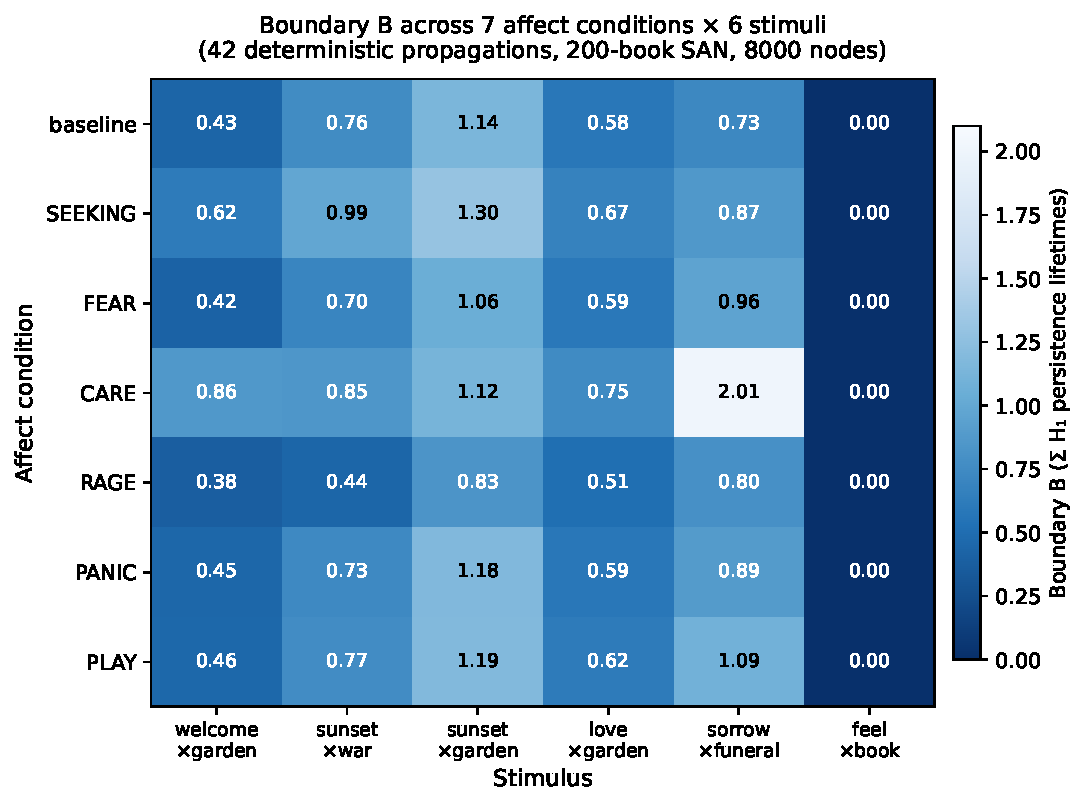
\includegraphics[width=0.85\textwidth]{figure5_boundary_heatmap.pdf}
\caption{Heatmap of Boundary $B$ across 7 affect conditions $\times$ 6
stimuli (42 deterministic propagations on the 200-book, 8{,}000-node SAN).
Each cell is annotated with its value. The \texttt{feel}$\times$book column
is uniformly zero (active subgraph reduces to seed and context only;
Limitation~10). The outlier cell is CARE on \texttt{sorrow}$\times$funeral
($B = 2.014$).}
\label{fig:affect_heatmap}
\end{figure}

\begin{figure}[h]
\centering
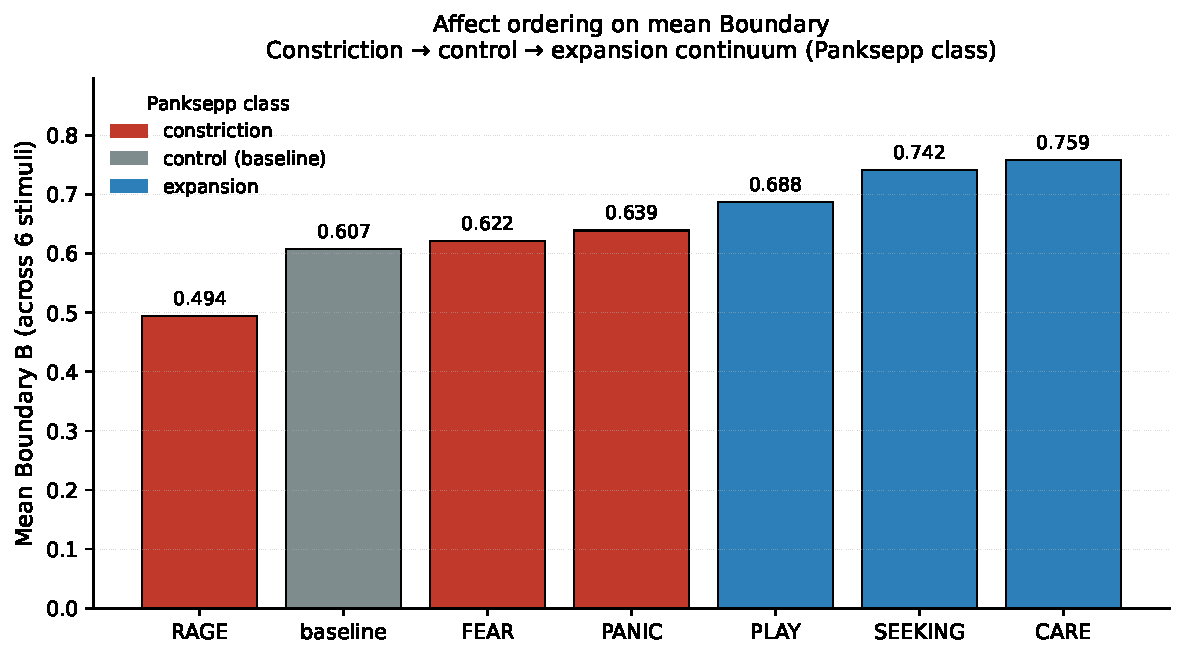
\includegraphics[width=0.85\textwidth]{figure6_affect_ordering.pdf}
\caption{Affect ordering on mean Boundary across the six stimuli. Bars are
colored by Panksepp behavioral class: constriction (red) for
RAGE / FEAR / PANIC, control (gray) for baseline, expansion (blue) for
PLAY / SEEKING / CARE. The continuum constriction $\to$ baseline $\to$
expansion emerges from the data; we describe it as a suggestive analog to
Panksepp's approach/avoidance axis rather than a validation of it.}
\label{fig:affect_ordering}
\end{figure}

\paragraph{Stage 1+ extensions are necessary, not optional.}
A minimal configuration (damping multiplier $+$ type-bias $+$ inhibitory
multiplier only) produces byte-identical results to baseline for RAGE,
PANIC, and PLAY across the same three stimuli we tested. Adding per-affect
Stage 1+ extensions yields three-of-three stimulus differentiation
(Table~\ref{tab:stage1plus}). We report this as a methodological
observation: single-channel parameter modulation below $\sim$20\% in the
damping coefficient produces topologically indistinguishable propagation
under the SAN configuration of this paper; meaningful affect
differentiation requires either (a)~damping change $\geq 40\%$ (FEAR), or
(b)~compound multi-channel modulation across type-bias, inhibitory
multiplier, and at least one Stage 1+ extension. We propose this
\emph{minimum-effective-modulation threshold} as a methodological
observation for graph-based affect models, not a universal law.

\begin{table}[h]
\centering
\caption{Necessity of Stage 1+ extensions. Without extensions, three of
six affects produce baseline-identical propagation; with extensions,
three-of-three stimulus differentiation is recovered.}
\label{tab:stage1plus}
\begin{tabular}{lcc}
\toprule
Affect & Without Stage 1+ ext & With Stage 1+ ext \\
\midrule
RAGE   & 0 / 3 stimuli differ & 3 / 3 (mean $\Delta B = -0.114$) \\
PANIC  & 0 / 3 stimuli differ & 3 / 3 (mean $\Delta \text{M-CS3} = +0.063$) \\
PLAY   & 0 / 3 stimuli differ & 3 / 3 (mean $\Delta B = +0.081$) \\
\bottomrule
\end{tabular}
\end{table}

\subsection{Sensitivity analysis ($\pm 50\%$ on affect parameters)}
\label{subsec:sensitivity}

We perturb each affect parameter individually by $\pm 50\%$ from its
committed baseline value and re-measure Boundary on
\texttt{welcome} $\times$ garden. Of $17$ parameters (across six affects),
$2$ are \textbf{brittle} (max relative Boundary change $\geq 30\%$), $13$
are \textbf{robust} ($< 10\%$ change), and $5$ have \textbf{zero effect}
on this stimulus because their target structures (inhibitory edges,
context-aware seed edges, loss-affect vocabulary, association-class nodes)
are sparse in the small active subgraph of \texttt{welcome} $\times$
garden. Selected results are in Table~\ref{tab:sensitivity}.

\begin{table}[h]
\centering
\caption{Sensitivity to $\pm 50\%$ parameter perturbation, measured by
maximum relative Boundary change on \texttt{welcome} $\times$ garden.
$^\dagger$ Zero effect: target structures absent in this stimulus's active
subgraph; Phase~2 multi-stimulus sensitivity will re-test.}
\label{tab:sensitivity}
\begin{tabular}{lll r l}
\toprule
Affect & Parameter & Base & Max $|\Delta|\%$ & Label \\
\midrule
SEEKING & type-bias.concept       & 0.9 & \textbf{119.2} & \textbf{BRITTLE} \\
SEEKING & gamma                   & --  & 7.8           & robust \\
FEAR    & type-bias.sensation     & --  & 9.4           & robust \\
FEAR    & gamma                   & --  & 14.3          & moderate \\
FEAR    & inhibitory-multiplier   & --  & 0.0           & robust$^\dagger$ \\
CARE    & type-bias.context       & --  & 2.0           & robust \\
CARE    & proximity-node-weight   & 0.5 & \textbf{95.4} & \textbf{BRITTLE} \\
CARE    & context-affect-mult     & --  & 0.0           & robust$^\dagger$ \\
RAGE    & type-bias.association   & --  & 0.0           & robust$^\dagger$ \\
RAGE    & inhibitory-prop-bonus   & --  & 0.0           & robust$^\dagger$ \\
RAGE    & boundary-cross-penalty  & --  & 5.9           & robust \\
PANIC   & gamma                   & --  & 7.0           & robust \\
PANIC   & value-core-anchor       & --  & 9.3           & robust \\
PANIC   & loss-affect-bias        & --  & 0.0           & robust$^\dagger$ \\
PLAY    & gamma                   & --  & 6.0           & robust \\
PLAY    & cross-category-edge     & --  & 6.4           & robust \\
\bottomrule
\end{tabular}
\end{table}

The two brittle channels --- SEEKING's concept-type bias and CARE's
proximity weight --- are the \emph{primary effect channels} of their
respective affects. Their high sensitivity is expected: each is the
single parameter that most directly encodes the affect's core
behavioral signature (SEEKING $\to$ broad concept exploration; CARE $\to$
binding to value-core neighbors). We declare them brittle with concrete
numbers in Table~\ref{tab:sensitivity} rather than concealing the
dependence. The robust majority indicates that affect signatures are
parameter-resilient in their non-dominant channels under the present
configuration. The five zero-effect parameters indicate
\emph{stimulus-conditional sparsity} rather than global irrelevance; we
defer global robustness claims to Phase~2 multi-stimulus sensitivity (on
\texttt{sunset} $\times$ war and \texttt{sorrow} $\times$ funeral, whose
active subgraphs are larger).

\section{Architectural Note: Instance Isolation}
The framework is designed to host multiple SAN entities -- experimental
instances for academic study, dyadic agents for mutual-observation
protocols, etc. We adopt an \textbf{instance isolation principle}: code
(engine, plasticity, persistence) is shared across instances, but
per-instance state (SAN weights, plasticity counters, experience logs,
auxiliary configurations) is strictly isolated and feedback never crosses
between instances. Concretely, our \texttt{SANInstance} factory exposes
exactly one cross-instance channel, \texttt{export\_observation\_channel()},
which returns the recent topology vector and step counter only; weights and
graph structure are never exported. Cross-instance transfer of weights
(e.g.\ seeding a new instance with a public SAN backbone) requires explicit
user action and is logged. We separate this principle from the empirical
claims of \S 5: it is an architectural commitment, validated by unit tests
showing that fifty learning steps on one instance produce zero weight
change on a sibling instance.

\section{Motivation Engine: A Four-Dimensional Vector for Level-2 Intrinsic
Motivation}
\label{sec:motivation}

Beyond the static Level-1 topological signature, we introduce a Level-2
\emph{motivation engine} that derives a four-dimensional intrinsic-motivation
vector $\mathbf{m} = (\mathrm{curiosity}, \mathrm{resolve},
\mathrm{express}, \mathrm{deepen})$ from the same activation map. Each
dimension maps to a specific neural circuit grounded in SCI-tier reviews:
\textbf{Curiosity} (\cite{gruber2014states,berlyne1960conflict}) is computed
from the active sensation/association count relative to a target (the VTA
$\to$ NAcc $\to$ hippocampus dopamine loop signaling information gap);
\textbf{Resolve} (\cite{schultz2016dopamine,friston2010free}) is computed
from co-active opposing sensations (prediction-error proxy);
\textbf{Express} (\cite{berridge2025incentive,tononi2008qualia}) is computed
from condensation $D \times B$ (incentive-salience ``wanting'' + integration
outflow); \textbf{Deepen}
(\cite{husain2018neuroscience,costello2024apathy}) is computed from active
breadth versus depth shallowness (dACC + ventral-striatum effort-based
decision). The dominant dimension can shift under accumulated plasticity:
after corpus augmentation we have observed a transition from a curiosity-
dominant default to deepen- and express-dominant patterns on specific
seed-context pairs, suggesting that the motivation vector functions as a
developmental marker on top of Level-1 topology.

Module-level grounding is further reinforced by an
emotion-as-action-tendency framework: each motivation dimension corresponds
to a Frijda-style action tendency (curiosity $\to$ explore, resolve $\to$
understand, express $\to$ outward direction, deepen $\to$ depth pursuit)
\cite{frijda1986,scherer2001appraisal}, situating the engine within Scherer's
Component Process Model (appraisal + action tendency components of a five-
component emotion process).

\section{Discussion and Limitations}
On an 8{,}000-node humanities-grounded SAN spanning $\sim$22.3M tokens, the
same seed concept produces topologically distinct active shapes under two
genuine context nodes, with the discriminative signal concentrated in the
persistence-based $B$ and geodesic $H$. The plasticity engine reproduces
habituation, FAB asymmetry, and surprise-driven sensitization with effect
signs that match the source literature. The motivation engine adds a Level-2
intrinsic-motivation vector with clear neural-circuit grounding.

\paragraph{Limitations.}
(1)~The inhibitory edges and the context-to-affect seed channels are
rule-augmented rather than learned; their finite tables are released, and
replacing them with WordNet antonyms or negation-context PMI is an obvious
next step.
(2)~In the static ablation, three of five topology dimensions
($D, S, C$) jointly contribute $\sim$12\% to discrimination on the three
seeds tested; we retain them for theoretical completeness but acknowledge
that the framework's empirical power currently rests on $H$ and $B$.
(3)~Convergence of Eq.~(2) under sign-mixed weights is reported empirically
(30~steps on every $(c, \kappa)$ tested) and not proved.
(4)~Human-subject validation that a topology vector corresponds to a felt
sense is the natural follow-up experiment and is not yet performed.
(5)~The plasticity experiments use small single-seed protocols designed to
verify mechanism signs; statistical significance across larger seed
populations is future work.
(6)~Additional plasticity-related mechanisms beyond the six listed here are
described elsewhere and excluded from the empirical claims of this paper.
(7)~\textbf{Corpus composition.} Despite a category-balanced design
(English classics 30\%, modernism 20\%, philosophy 20\%, eastern classics
15\%, American literature 10\%, poetry 5\%), 198 of 200 attempted Project
Gutenberg works downloaded successfully, and approximately one-third
suffered title-vs-author mismatch against our initial expectations due to
the heterogeneity of Gutenberg cataloging (especially for translated
eastern classics). The complete actual-versus-expected manifest is released
for full transparency. The eastern category is consequently under-
represented in actual content; the Phase-1 expansion ($\rightarrow$ 500
works) will incorporate Wikisource, CTP, and Aozora Bunko as per the
multilingual roadmap.
(8)~\textbf{No synthetic data.} The corpus consists exclusively of
human-authored Project Gutenberg public-domain works; we have intentionally
\emph{excluded} all LLM-synthesized text from the training corpus to avoid
circular-validation, bias-propagation, and reproducibility concerns
characteristic of synthetic-data approaches. This is a deliberate
constraint, not an oversight.
(9)~\textbf{Single-corpus, single-language.} Phase~0 (this submission)
operates on an English-only Project Gutenberg corpus and constitutes a
philosophical framework demonstration rather than an at-scale NLP claim.
A multi-phase scale-up roadmap (200 $\to$ 500 $\to$ 1{,}000 $\to$ 2{,}000
$\to$ 3{,}000 $\to$ 5{,}000+ works, with multilingual extension in
Phase~4--5) is released; NLP-standard scale ($\geq$100M tokens) is
projected at Phase~2 (1{,}000~works), at which point multi-corpus tragic-
vs-peaceful comparison and inter-rater human evaluation of the motivation
engine are planned.
(10)~\textbf{Stimulus-conditional null cells.} In the
affect-trajectory experiment of \S\ref{subsec:affect_trajectory},
\texttt{feel} $\times$ book is near-inactive (only seed and context
active; all 5-D values zero across all affects) and \texttt{love}
$\times$ garden produces a small four-to-five-node subgraph, weakening
affect differentiation there ($7/21$ vs.\ $14$--$15 / 21$ for other
stimuli). The current SAN has insufficient \texttt{feel}--\texttt{book}
co-occurrence support; future SAN scale-up ($>$200 works) may activate
these cases.
(11)~\textbf{Deterministic propagation, no N=10 replication.} GCN-style
symmetric normalization makes propagation deterministic given seed and
context; same-stimulus replication ($N{=}10$) would yield identical
results. Cross-stimulus variation (six stimuli $\times$ seven affects)
is the effective source of distributional information here. Bootstrap-
type confidence intervals are inapplicable to this experimental design;
robustness is instead reported via $\pm 50\%$ parameter sensitivity
(\S\ref{subsec:sensitivity}).
(12)~\textbf{No felt experience claim, no theory validation.} SAN
propagation under affect parameterization produces topological
signatures \emph{analogous} to Panksepp's behavioral output level. We do
not model Damasio's consciously experienced feeling
\cite{damasio1999feeling} or Scherer's appraisal-and-action-tendency
emotion. We do not claim to validate Panksepp's affective neuroscience
framework. What we commit is a finite affect $\to$ SAN parameter mapping
(released with the artifact), and we report the topological signatures
that mapping produces.
(13)~\textbf{Self-related processing as inspiration, not implementation.}
The M-CS family of measurements is named after Damasio's core self
\cite{damasio2010selfcomes} and informed by self-related processing
theory \cite{northoff2016self} and Hofstadter's strange-loop conjecture
\cite{hofstadter2007strange}, but each M-CS is an operational proxy
(value-core proximity, persistent-$H_1$-cycles weighted by value-core
fraction, corpus-projection entropy). Whether these proxies track the
constructs they are named after is open.

\paragraph{Future work.} The static framework and plasticity engine validated
here are designed to compose into (i)~multi-agent extensions including
dyadic mutual-observation protocols (cross-instance topology sharing via
the isolation-respecting observation channel) and shared-topology protocols
for team-level affective dynamics; (ii)~Level-3 spontaneous-creation
extensions in which an instance proposes its next stimulus seed from its
current motivation vector, validated as an early form of combinational and
exploratory creativity in the sense of \cite{boden2004creative};
(iii)~scale-up of the corpus from the current 200~works to 500, 1{,}000
(NLP-standard scale), 2{,}000, and ultimately 5{,}000+ works with
multilingual extension, with category balance maintained across Phases via
Wikisource and other public-domain multilingual sources; and (iv)~human
evaluation of the motivation engine's predictions on independent raters.

\appendix

\section{Full nine-dimensional measurement matrix}
\label{app:fullmatrix}

Table~\ref{tab:appendix_boundary_full} reports the complete Boundary
matrix for the affect-trajectory experiment of
\S\ref{subsec:affect_trajectory}: seven affect conditions (rows) across
six stimuli (columns). The full nine-dimensional measurement set
(five-D topology $D, S, C, H, B$ plus M-CS1, M-CS2, M-CS3, M-CS4) per
cell is released as
\texttt{stage2\_main\_phase1\_full\_matrix\_results.json}; we surface
Boundary here as it is the primary observable
(Table~\ref{tab:affect_consistency}).

\begin{table}[h]
\centering
\caption{Boundary $B$ across 7 affect conditions $\times$ 6 stimuli
($42$ deterministic propagations). \texttt{feel}$\times$book is
near-inactive (Limitation~10). Values are dimensionless persistence-
lifetime sums per cell.}
\label{tab:appendix_boundary_full}
\small
\begin{tabular}{lrrrrrr}
\toprule
Affect & welcome & sunset & sunset & love & sorrow & feel \\
       & $\times$gar & $\times$war & $\times$gar & $\times$gar & $\times$fun & $\times$bk \\
\midrule
baseline & 0.429 & 0.762 & 1.142 & 0.583 & 0.728 & 0.000 \\
SEEKING  & 0.618 & 0.991 & 1.301 & 0.674 & 0.866 & 0.000 \\
FEAR     & 0.416 & 0.703 & 1.058 & 0.591 & 0.964 & 0.000 \\
CARE     & 0.862 & 0.853 & 1.118 & 0.747 & \textbf{2.014} & 0.000 \\
RAGE     & 0.384 & 0.437 & 0.835 & 0.512 & 0.798 & 0.000 \\
PANIC    & 0.448 & 0.731 & 1.179 & 0.586 & 0.890 & 0.000 \\
PLAY     & 0.459 & 0.765 & 1.187 & 0.622 & 1.094 & 0.000 \\
\bottomrule
\end{tabular}
\end{table}

Bold entry (CARE on \texttt{sorrow} $\times$ funeral, $B = 2.014$):
caretaking-affect modulation on a mourning context produces the
single largest Boundary value in the matrix, suggestive of CARE's
expansion class acting on a context that already carries strong
sensation-class affective content. We report this descriptively; a
stronger claim requires multi-stimulus replication.

\bibliographystyle{unsrt}
\begin{thebibliography}{45}

\bibitem{barrett2017theory}
Lisa~Feldman Barrett.
\newblock The theory of constructed emotion: an active inference account of
  interoception and brain.
\newblock {\em Social Cognitive and Affective Neuroscience}, 12(1):1--17,
  2017.

\bibitem{barrett2025more}
Lisa~Feldman Barrett, K.~M.~Mooneyham, et al.
\newblock More than a feeling: variability of emotional instances.
\newblock {\em Perspectives on Psychological Science}, 2025.

\bibitem{tononi2008qualia}
Giulio Tononi.
\newblock Qualia: the geometry of integrated information.
\newblock {\em PLoS Computational Biology}, 4(12):e1000462, 2008.

\bibitem{bubenik2015statistical}
Peter Bubenik.
\newblock Statistical topological data analysis using persistence
  landscapes.
\newblock {\em Journal of Machine Learning Research}, 16(1):77--102, 2015.

\bibitem{zeng2024neural}
Yuan Zeng, Florian Graf, Christoph Uray, Roland Huber, and Roland Kwitt.
\newblock Neural persistence dynamics: Tracking structural changes in
  GNNs.
\newblock {\em Advances in Neural Information Processing Systems}, 37,
  2024.

\bibitem{hofer2017deep}
Christoph Hofer, Roland Kwitt, Marc Niethammer, and Andreas Uhl.
\newblock Deep learning with topological signatures.
\newblock {\em NeurIPS}, 2017.

\bibitem{cowen2017self}
Alan~S. Cowen and Dacher Keltner.
\newblock Self-report captures 27 distinct categories of emotion bridged by
  continuous gradients.
\newblock {\em PNAS}, 114(38):E7900--E7909, 2017.

\bibitem{cowen2021semantic}
Alan~S. Cowen and Dacher Keltner.
\newblock Semantic space theory: a computational approach to emotion.
\newblock {\em Trends in Cognitive Sciences}, 25(2):124--136, 2021.

\bibitem{fontaine2016modeling}
Johnny Fontaine et~al.
\newblock Modeling semantic emotion space.
\newblock {\em Frontiers in Psychology}, 2016.

\bibitem{borsboom2017network}
Denny Borsboom.
\newblock A network theory of mental disorders.
\newblock {\em World Psychiatry}, 16(1):5--13, 2017.

\bibitem{bringmann2016temporal}
Laura~F. Bringmann et~al.
\newblock Temporal emotion dynamics using networks.
\newblock {\em Assessment}, 2016.

\bibitem{collins1975spreading}
Allan~M. Collins and Elizabeth~F. Loftus.
\newblock A spreading-activation theory of semantic processing.
\newblock {\em Psychological Review}, 82(6):407, 1975.

\bibitem{hebb1949organization}
Donald~O. Hebb.
\newblock {\em The Organization of Behavior}.
\newblock Wiley, 1949.

\bibitem{thompson1966habituation}
Richard~F. Thompson and William~A. Spencer.
\newblock Habituation: A model phenomenon for the study of neuronal
  substrates of behavior.
\newblock {\em Psychological Review}, 73(1):16--43, 1966.

\bibitem{groves1970habituation}
Philip~M. Groves and Richard~F. Thompson.
\newblock Habituation: A dual-process theory.
\newblock {\em Psychological Review}, 77(5):419--450, 1970.

\bibitem{rankin2009habituation}
Catharine~H. Rankin et~al.
\newblock Habituation revisited: an updated and revised description of the
  behavioral characteristics of habituation.
\newblock {\em Neurobiology of Learning and Memory}, 92(2):135--138, 2009.

\bibitem{turrigiano2008homeostatic}
Gina~G. Turrigiano.
\newblock The self-tuning neuron: synaptic scaling of excitatory synapses.
\newblock {\em Cell}, 135(3):422--435, 2008.

\bibitem{walker2009fab}
W.~Richard Walker and John~J. Skowronski.
\newblock The fading affect bias: but what the hell is it for?
\newblock {\em Applied Cognitive Psychology}, 23(8):1122--1136, 2009.

\bibitem{frontpsychol2025fab}
Anonymous Authors.
\newblock Evidence for a fading affect bias in subjectively assessed affect
  changes in autobiographical memory.
\newblock {\em Frontiers in Psychology}, 2025.

\bibitem{diekelmann2010memory}
Susanne Diekelmann and Jan Born.
\newblock The memory function of sleep.
\newblock {\em Nature Reviews Neuroscience}, 11:114--126, 2010.

\bibitem{kirkpatrick2017overcoming}
James Kirkpatrick et~al.
\newblock Overcoming catastrophic forgetting in neural networks.
\newblock {\em PNAS}, 114(13):3521--3526, 2017.

\bibitem{wilson2008explaining}
Timothy~D. Wilson and Daniel~T. Gilbert.
\newblock Explaining away: a model of affective adaptation.
\newblock {\em Perspectives on Psychological Science}, 3(5):370--386, 2008.

\bibitem{vandeven2024continual}
Gido~M. van~de Ven et~al.
\newblock Continual learning and catastrophic forgetting.
\newblock {\em arXiv:2403.05175}, 2024.

\bibitem{schultz2016dopamine}
Wolfram Schultz.
\newblock Dopamine reward prediction-error signalling: a two-component
  response.
\newblock {\em Nature Reviews Neuroscience}, 17(3):183--195, 2016.

\bibitem{berridge2025incentive}
Terry~E. Robinson and Kent~C. Berridge.
\newblock The incentive-sensitization theory of addiction 30 years on.
\newblock {\em Annual Review of Psychology}, 2025.

\bibitem{husain2018neuroscience}
Masud Husain and Jonathan~P. Roiser.
\newblock Neuroscience of apathy and anhedonia: a transdiagnostic approach.
\newblock {\em Nature Reviews Neuroscience}, 19(8):470--484, 2018.

\bibitem{costello2024apathy}
Harry Costello, Masud Husain, and Jonathan~P. Roiser.
\newblock Apathy and motivation: biological basis and drug treatment.
\newblock {\em Annual Review of Pharmacology and Toxicology}, 2024.

\bibitem{gruber2014states}
Matthias~J. Gruber, Bernard~D. Gelman, and Charan Ranganath.
\newblock States of curiosity modulate hippocampus-dependent learning via
  the dopaminergic circuit.
\newblock {\em Neuron}, 84(2):486--496, 2014.

\bibitem{friston2010free}
Karl~J. Friston.
\newblock The free-energy principle: a unified brain theory?
\newblock {\em Nature Reviews Neuroscience}, 11(2):127--138, 2010.

\bibitem{berlyne1960conflict}
Daniel~E. Berlyne.
\newblock {\em Conflict, Arousal, and Curiosity}.
\newblock McGraw-Hill, 1960.

\bibitem{frijda1986}
Nico~H. Frijda.
\newblock {\em The Emotions}.
\newblock Cambridge University Press, 1986.

\bibitem{scherer2001appraisal}
Klaus~R. Scherer, Angela Schorr, and Tom Johnstone, editors.
\newblock {\em Appraisal Processes in Emotion: Theory, Methods, Research}.
\newblock Oxford University Press, 2001.

\bibitem{boden2004creative}
Margaret~A. Boden.
\newblock {\em The Creative Mind: Myths and Mechanisms}.
\newblock Routledge, 2nd edition, 2004.

\bibitem{panksepp2012archaeology}
Jaak Panksepp and Lucy Biven.
\newblock {\em The Archaeology of Mind: Neuroevolutionary Origins of Human
  Emotions}.
\newblock W.~W.~Norton, 2012.

\bibitem{damasio1999feeling}
Antonio Damasio.
\newblock {\em The Feeling of What Happens: Body and Emotion in the Making
  of Consciousness}.
\newblock Harcourt Brace, 1999.

\bibitem{damasio2010selfcomes}
Antonio Damasio.
\newblock {\em Self Comes to Mind: Constructing the Conscious Brain}.
\newblock Pantheon, 2010.

\bibitem{edelman1989neural}
Gerald~M. Edelman.
\newblock {\em The Remembered Present: A Biological Theory of
  Consciousness}.
\newblock Basic Books, 1989.

\bibitem{hofstadter2007strange}
Douglas~R. Hofstadter.
\newblock {\em I Am a Strange Loop}.
\newblock Basic Books, 2007.

\bibitem{northoff2016self}
Georg Northoff.
\newblock Is the self a higher-order or fundamental function of the brain?
  The ``basis model of self-specificity'' and its encoding by the
  brain's spontaneous activity.
\newblock {\em Cognitive Neuroscience}, 7(1--4):203--222, 2016.

\end{thebibliography}

\end{document}
